\documentclass[12pt,a4paper]{article}

% ─── Page Layout ───────────────────────────────────────────────────────────────
\usepackage[a4paper, margin=0.8in, headheight=14pt]{geometry}

% ─── Fonts (XeLaTeX) ───────────────────────────────────────────────────────────
\usepackage{fontspec}
\usepackage{unicode-math}
\setmainfont{TeX Gyre Pagella}
\setmonofont[Scale=0.88]{TeX Gyre Cursor}
\setmathfont{Latin Modern Math}

% ─── Packages ──────────────────────────────────────────────────────────────────
\usepackage{xcolor}
\usepackage{colortbl}
\usepackage{titlesec}
\usepackage{enumitem}
\usepackage{tabularx}
\usepackage{booktabs}
\usepackage{array}
\usepackage{amsmath}
\usepackage{tikz}
\usetikzlibrary{shapes.geometric, arrows.meta, positioning, calc, fit, decorations.pathreplacing}
\usepackage{tcolorbox}
\tcbuselibrary{skins, breakable}
\usepackage{hyperref}
\usepackage{fancyhdr}
\usepackage{graphicx}
\usepackage{microtype}
\hyphenpenalty=10000
\exhyphenpenalty=10000
\sloppy
\usepackage{caption}
\usepackage{setspace}
\usepackage{multirow}
\usepackage{tocloft}

% ─── Q&A helper ────────────────────────────────────────────────────────────────
\newcommand{\Q}[1]{\textbf{#1}\par\noindent\ignorespaces}

% ─── Colour Palette ────────────────────────────────────────────────────────────
\definecolor{myred}{RGB}{196,30,58}
\definecolor{mydark}{RGB}{30,30,50}
\definecolor{mygreen}{RGB}{14,120,80}
\definecolor{myteal}{RGB}{0,130,140}
\definecolor{myamber}{RGB}{180,100,0}
\definecolor{mypurple}{RGB}{100,30,160}
\definecolor{mygray}{RGB}{246,247,249}
\definecolor{mgframe}{RGB}{180,185,200}
\definecolor{watermark}{RGB}{145,150,170}
\definecolor{hdrred}{RGB}{250,232,235}
\definecolor{hdrgreen}{RGB}{220,244,233}
\definecolor{hdrteal}{RGB}{220,242,244}
\definecolor{hdramber}{RGB}{253,242,215}
\definecolor{hdrpurple}{RGB}{238,228,255}
\definecolor{hdrgray}{RGB}{238,240,245}
\definecolor{rowalt}{RGB}{250,251,253}

% ─── Section Formatting ────────────────────────────────────────────────────────
\titleformat{\section}
  {\large\bfseries\color{myred}}{\thesection.}{0.5em}{}
  [\vspace{1pt}{\color{myred}\rule{\linewidth}{0.8pt}}]
\titleformat{\subsection}
  {\normalsize\bfseries\color{myteal}}{\thesubsection}{0.5em}{}
\titlespacing*{\section}{0pt}{18pt}{7pt}
\titlespacing*{\subsection}{0pt}{11pt}{4pt}

% ─── Paragraph ─────────────────────────────────────────────────────────────────
\setlength{\parindent}{0pt}
\setlength{\parskip}{4pt}

% ─── TOC Styling ───────────────────────────────────────────────────────────────
\renewcommand{\cfttoctitlefont}{\large\bfseries\color{myred}}
\renewcommand{\cftaftertoctitle}{\par\noindent{\color{myred}\rule{\linewidth}{0.8pt}}}
\setlength{\cftbeforetoctitleskip}{0pt}
\setlength{\cftaftertoctitleskip}{6pt}
\renewcommand{\cftsecfont}{\normalsize\bfseries\color{mydark}}
\renewcommand{\cftsecpagefont}{\normalsize\bfseries\color{mydark}}
\renewcommand{\cftsecleader}{\cftdotfill{\cftdotsep}}
\setlength{\cftbeforesecskip}{7pt}
\renewcommand{\cftsubsecfont}{\small\color{mydark}}
\renewcommand{\cftsubsecpagefont}{\small\color{mydark}}
\setlength{\cftbeforesubsecskip}{3pt}
\setlength{\cftsubsecindent}{1.4em}

% ─── Table helpers ─────────────────────────────────────────────────────────────
\renewcommand{\arraystretch}{1.45}
\setlength{\tabcolsep}{6pt}
\arrayrulecolor{mydark}
\newcolumntype{B}[1]{>{\small\bfseries\raggedright\arraybackslash}m{#1}}
\newcolumntype{Y}{>{\small\raggedright\arraybackslash}X}
\renewcommand{\tabularxcolumn}[1]{m{#1}}

% ─── Header / Footer ───────────────────────────────────────────────────────────
\pagestyle{fancy}
\fancyhf{}
\fancyhead[L]{\small\color{myred}\textbf{PE-EC703B}\;\color{mydark}--- Wireless Sensor Networks}
\fancyhead[R]{\small\color{myteal}\textbf{Module 5 Notes}}
\fancyfoot[C]{\small\color{mydark}\thepage}
\fancyfoot[R]{\small\color{watermark}\textit{\copyright\ Biraj}}
\renewcommand{\headrulewidth}{0.5pt}
\renewcommand{\footrulewidth}{0.3pt}

% ─── Hyperref ──────────────────────────────────────────────────────────────────
\hypersetup{
  colorlinks=true, linkcolor=myteal, urlcolor=myteal,
  pdfauthor={Biraj Sarkar},
  pdftitle={PE-EC703B --- Module 5 Notes}
}

% ─── tcolorbox styles ──────────────────────────────────────────────────────────
\tcbset{
  tikzbox/.style={
    colback=mygray, colframe=mgframe, boxrule=0.6pt, arc=4pt,
    left=8pt, right=8pt, top=6pt, bottom=6pt,
    colbacktitle=mgframe, coltitle=mydark,
    fonttitle=\small\bfseries
  },
  defbox/.style={
    colback=hdrgreen, colframe=mygreen, boxrule=0.8pt, arc=4pt,
    left=9pt, right=9pt, top=6pt, bottom=6pt,
    colbacktitle=mygreen, coltitle=white,
    fonttitle=\small\bfseries
  },
  formulabox/.style={
    colback=hdrteal, colframe=myteal, boxrule=0.8pt, arc=4pt,
    left=9pt, right=9pt, top=7pt, bottom=7pt,
    colbacktitle=myteal, coltitle=white,
    fonttitle=\small\bfseries
  },
  examplebox/.style={
    colback=hdramber, colframe=myamber, boxrule=0.8pt, arc=4pt,
    left=9pt, right=9pt, top=6pt, bottom=6pt,
    colbacktitle=myamber, coltitle=white,
    fonttitle=\small\bfseries
  },
  masonbox/.style={
    colback=hdrpurple, colframe=mypurple, boxrule=0.8pt, arc=4pt,
    left=9pt, right=9pt, top=6pt, bottom=6pt,
    colbacktitle=mypurple, coltitle=white,
    fonttitle=\small\bfseries
  },
  exambox/.style={
    colback=hdrpurple, colframe=mypurple, boxrule=1pt, arc=5pt,
    left=10pt, right=10pt, top=8pt, bottom=8pt,
    colbacktitle=mypurple, coltitle=white,
    fonttitle=\bfseries,
    breakable, title after break={\textbf{Frequently Asked / Viva Questions (contd.)}}}
}
\tcbset{breakable}

% ─── TikZ styles ───────────────────────────────────────────────────────────────
\tikzset{
  block/.style={rectangle, draw=myteal, fill=hdrteal,
    text width=2.4cm, align=center, minimum height=0.95cm,
    font=\small, rounded corners=3pt, line width=0.7pt},
  redblock/.style={rectangle, draw=myred, fill=hdrred,
    text width=2.4cm, align=center, minimum height=0.95cm,
    font=\small, rounded corners=3pt, line width=0.7pt},
  netnode/.style={rectangle, draw=myteal, fill=hdrteal,
    text width=1.5cm, align=center, minimum height=0.8cm,
    font=\small, rounded corners=3pt, line width=0.7pt},
  sumjunc/.style={circle, draw=myamber, fill=hdramber,
    minimum size=0.62cm, font=\small, line width=0.8pt},
  snode/.style={circle, draw=mypurple, fill=hdrpurple,
    minimum size=0.55cm, font=\footnotesize, line width=0.7pt},
  arrow/.style={-Stealth, thick, color=mydark},
  redarrow/.style={-Stealth, thick, color=myred},
  line/.style={thick, color=mydark}
}

% ═══════════════════════════════════════════════════════════════════════════════
\begin{document}
% ═══════════════════════════════════════════════════════════════════════════════

\begin{center}
  {\LARGE\bfseries\color{myred} PE-EC703B --- Wireless Sensor Networks}\\[5pt]
  {\normalsize\color{mydark} Semester VII \quad$\bullet$\quad 3L:0T:0P \quad$\bullet$\quad 3 Credits}\\[3pt]
  {\normalsize\color{myteal}\textbf{Module 5 Exam Notes: Design Principles, Gateway Concepts \& TinyOS/nesC}}\\[3pt]
  {\small\color{mydark} CGEC \;$|$\; B.Tech ECE (2023--27) \;$|$\; \textit{Biraj Sarkar}}
\end{center}
\vspace{2pt}
\noindent{\color{myred}\rule{\linewidth}{1.5pt}}
\vspace{2pt}

\hypersetup{linkcolor=mydark}
\tableofcontents
\hypersetup{linkcolor=myteal}
\newpage

% ===============================================================================
\section{Design Principles for Wireless Sensor Networks}
% ===============================================================================

WSN design is fundamentally different from traditional network design. The scarcity of energy, computation, and memory requires application-aware, cross-layer, and energy-first design principles.

\begin{tcolorbox}[formulabox, title={\textbf{Core WSN Design Principles}}]
\begin{enumerate}[leftmargin=*, itemsep=5pt]
  \item \textbf{Energy efficiency first:} Every design decision --- protocol, algorithm, hardware --- must minimize energy consumption. Network lifetime is the primary performance metric. Aggressive duty cycling (radio sleep), in-network processing, and shortest-path routing are non-negotiable.

  \item \textbf{In-network processing (data-centric design):} Perform aggregation, filtering, and fusion inside the network, not just at the sink. A cluster head that averages 10 readings saves $9\times$ the transmission energy of forwarding raw data.

  \item \textbf{Cross-layer design:} Traditional layered (OSI) design isolates layers. WSN protocols jointly optimize MAC + routing + application (e.g., LEACH combines clustering at the network layer with TDMA at the MAC layer, driven by application data rate).

  \item \textbf{Self-organization and adaptivity:} The network must configure itself, elect cluster heads, discover routes, and heal from failures without human intervention. Protocols must work correctly under random deployment and topology changes.

  \item \textbf{Collaboration and redundancy:} Exploit spatial redundancy --- multiple nodes cover the same area. Use data from multiple sensors for reliability and accuracy (spatial diversity). Active nodes can cover for sleeping or dead nodes.

  \item \textbf{Data-centric communication:} Address data by its attributes (``temperature $> 40$°C''), not by node IDs. This enables in-network aggregation, suppression of duplicate data, and semantic routing.

  \item \textbf{Quality/fidelity trade-off:} Accept lower resolution or less frequent data in exchange for energy savings. Adaptive sampling reduces data rate when environment is stable, increases it during events.

  \item \textbf{Security by design:} Assume a hostile deployment environment. Build authentication and freshness into every protocol (not bolted on after). Use lightweight symmetric cryptography (AES-128) rather than public-key.
\end{enumerate}
\end{tcolorbox}

% ===============================================================================
\section{Gateway Concepts in WSN}
% ===============================================================================

\begin{tcolorbox}[defbox, title={\textbf{WSN Gateway --- Definition}}]
A \textbf{WSN gateway} is a device that bridges the wireless sensor network with an external network (such as the Internet, an enterprise LAN, or a cellular network). It performs \textbf{protocol translation} between the low-power WSN protocols (IEEE 802.15.4 / ZigBee) and standard IP networking (TCP/IP / HTTP).
\end{tcolorbox}

\subsection{Need for a Gateway}

\begin{itemize}[leftmargin=*, itemsep=3pt]
  \item WSN nodes speak IEEE 802.15.4 / ZigBee; the internet speaks TCP/IP. These are incompatible at multiple layers.
  \item Sensor nodes are too resource-constrained to run a full TCP/IP stack.
  \item The gateway provides a management interface for the WSN (task injection, firmware update, health monitoring).
  \item The gateway buffers data from the WSN and forwards to cloud/server in bursts, reducing WSN active time.
\end{itemize}

\subsection{Gateway Architecture and Functions}

\begin{tcolorbox}[tikzbox, title={WSN Gateway Integration Diagram}]
\centering
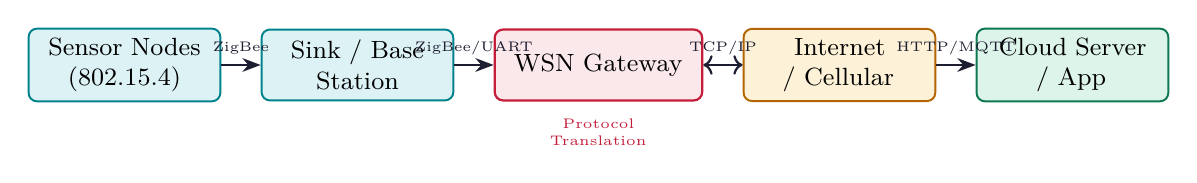
\begin{tikzpicture}[node distance=0.5cm and 0.9cm,
  wsblock/.style={rectangle, draw=myteal, fill=hdrteal, text width=2.2cm,
    align=center, minimum height=0.9cm, font=\small, rounded corners=3pt, line width=0.7pt},
  gwblock/.style={rectangle, draw=myred, fill=hdrred, text width=2.4cm,
    align=center, minimum height=0.9cm, font=\small, rounded corners=3pt, line width=0.8pt},
  ipblock/.style={rectangle, draw=myamber, fill=hdramber, text width=2.2cm,
    align=center, minimum height=0.9cm, font=\small, rounded corners=3pt, line width=0.7pt},
  srvblock/.style={rectangle, draw=mygreen, fill=hdrgreen, text width=2.2cm,
    align=center, minimum height=0.9cm, font=\small, rounded corners=3pt, line width=0.7pt}]

  % WSN side
  \node[wsblock] (sn) {Sensor Nodes (802.15.4)};
  \node[wsblock, right=0.5cm of sn] (sink) {Sink / Base Station};

  % Gateway
  \node[gwblock, right=0.5cm of sink] (gw) {WSN Gateway};

  % Internet
  \node[ipblock, right=0.5cm of gw] (inet) {Internet / Cellular};

  % Server / Cloud
  \node[srvblock, right=0.5cm of inet] (srv) {Cloud Server / App};

  % Arrows
  \draw[arrow] (sn) -- (sink) node[midway, above, font=\tiny] {ZigBee};
  \draw[arrow] (sink) -- (gw) node[midway, above, font=\tiny] {ZigBee/UART};
  \draw[arrow, <->] (gw) -- (inet) node[midway, above, font=\tiny] {TCP/IP};
  \draw[arrow] (inet) -- (srv) node[midway, above, font=\tiny] {HTTP/MQTT};

  % Gateway label
  \node[font=\tiny, color=myred, below=0.1cm of gw, align=center, text width=1.8cm] {Protocol Translation};
\end{tikzpicture}
\end{tcolorbox}

\textbf{Gateway functions:}
\begin{itemize}[leftmargin=*, itemsep=3pt]
  \item \textbf{Protocol translation:} Converts ZigBee/IEEE 802.15.4 frames to IP packets and vice versa.
  \item \textbf{Data buffering:} Stores sensor data locally (flash/SD card) if internet is unavailable.
  \item \textbf{Data formatting:} Converts raw sensor values to JSON, XML, or MQTT payloads for cloud APIs.
  \item \textbf{Security bridging:} Translates between WSN security (AES-128 with SNEP) and internet security (TLS/SSL).
  \item \textbf{Task injection:} Receives queries from the internet and injects them as interests into the WSN.
  \item \textbf{Network management:} Monitors WSN health, tracks node battery levels, and triggers alarms.
\end{itemize}

% ===============================================================================
\section{WSN to Internet Communication}
% ===============================================================================

\begin{tcolorbox}[defbox, title={\textbf{WSN-to-Internet Communication}}]
\textbf{WSN to Internet} communication refers to the uplink flow where sensor data is transported from the sensor field, through the gateway, to an Internet-connected server or cloud platform for storage, processing, and visualization.
\end{tcolorbox}

\subsection{Integration Approaches}

\par\noindent
{\renewcommand{\arraystretch}{1.5}%
\begin{tabularx}{\linewidth}{|B{3.2cm}|Y|Y|}
\hline
\textbf{Approach} & \textbf{Description} & \textbf{Protocols} \\
\hline
\textbf{Gateway-based (Overlay)} & WSN and Internet are two separate networks; gateway translates between them & ZigBee + HTTP/MQTT gateway \\
\hline
\textbf{6LoWPAN (IP-native)} & Runs IPv6 directly on IEEE 802.15.4 nodes using header compression; no separate gateway needed & 6LoWPAN + CoAP + RPL \\
\hline
\textbf{Middleware approach} & Software layer abstracts WSN heterogeneity; presents a uniform API to internet applications & REST-based middleware \\
\hline
\end{tabularx}}

\subsection{6LoWPAN (IPv6 over Low-Power Wireless PANs)}

\begin{tcolorbox}[defbox, title={\textbf{6LoWPAN --- Definition}}]
\textbf{6LoWPAN} is an IETF adaptation layer (RFC 4944) that enables \textbf{IPv6 packets to be transmitted over IEEE 802.15.4} networks by compressing IPv6 headers (from 40 bytes to 2--6 bytes) and fragmenting large packets to fit the 127-byte IEEE 802.15.4 frame. This allows sensor nodes to participate directly in the Internet of Things.
\end{tcolorbox}

\textbf{Key functions of 6LoWPAN adaptation layer:}
\begin{itemize}[leftmargin=*, itemsep=3pt]
  \item \textbf{Header compression:} IPv6 header (40 B) + UDP (8 B) compressed to $\leq$ 6 B using IPHC (IP Header Compression).
  \item \textbf{Fragmentation and reassembly:} IPv6 MTU = 1280 B; IEEE 802.15.4 payload = 102 B (max). 6LoWPAN fragments and reassembles.
  \item \textbf{Mesh addressing:} Supports multi-hop routing for IEEE 802.15.4 using mesh header.
  \item \textbf{Neighbor discovery:} Optimized ND for low-power, lossy networks (ND-LowPAN).
\end{itemize}

\subsection{CoAP (Constrained Application Protocol)}

\begin{tcolorbox}[defbox, title={\textbf{CoAP --- Definition}}]
\textbf{CoAP} is a lightweight application protocol designed for constrained IoT and WSN devices, functioning as the ``HTTP for IoT.'' It runs over UDP (instead of TCP), uses a REST-based request/response model, and supports GET, PUT, POST, DELETE operations on resources (sensor readings, actuator states).
\end{tcolorbox}

\begin{itemize}[leftmargin=*, itemsep=3pt]
  \item \textbf{Binary encoding:} Compact binary header (4 bytes fixed header vs HTTP's 100s of bytes).
  \item \textbf{UDP-based:} Avoids TCP's connection overhead and handshake energy cost.
  \item \textbf{Confirmable messages:} CoAP has its own reliability mechanism (CON messages with ACK).
  \item \textbf{Observe extension:} Server pushes updates to subscribed clients (no polling needed).
  \item \textbf{Gateway translation:} A CoAP-HTTP proxy converts between CoAP (sensor side) and HTTP (internet side).
\end{itemize}

% ===============================================================================
\section{Internet to WSN Communication}
% ===============================================================================

\begin{tcolorbox}[defbox, title={\textbf{Internet-to-WSN Communication}}]
\textbf{Internet to WSN} communication refers to the downlink flow: queries, commands, firmware updates, and configuration sent from an Internet-connected server or user application into the sensor network.
\end{tcolorbox}

\subsection{Challenges of Internet-to-WSN Downlink}
\begin{itemize}[leftmargin=*, itemsep=3pt]
  \item \textbf{Sleeping nodes:} Sensor nodes may be asleep when a command arrives. The gateway must buffer the command and deliver it at the node's next wake-up.
  \item \textbf{Asymmetric bandwidth:} Internet downlink can push data faster than the WSN can absorb.
  \item \textbf{Addressing:} Individual nodes may have only 16-bit short addresses (not globally routable). The gateway maps external requests to internal WSN addresses.
  \item \textbf{Reliability:} IEEE 802.15.4 is lossy; downlink commands may need retransmission.
\end{itemize}

\subsection{Mechanisms}
\begin{itemize}[leftmargin=*, itemsep=3pt]
  \item \textbf{MQTT (Message Queuing Telemetry Transport):} Publish-subscribe protocol over TCP; the broker buffers messages for offline sensor nodes. Gateway subscribes to topics and injects commands into WSN.
  \item \textbf{RPL (Routing Protocol for Low-Power and Lossy Networks):} IETF routing protocol for 6LoWPAN; builds a Destination-Oriented DAG (DODAG) from the sink downward, enabling Internet-initiated routes.
  \item \textbf{CoAP Observe:} Internet server registers observation on a sensor resource; sensor pushes updates. Reverse: server PUTs commands to sensor actuator resources.
\end{itemize}

% ===============================================================================
\section{Operating Systems for WSN}
% ===============================================================================

\begin{tcolorbox}[defbox, title={\textbf{WSN Operating System --- Requirements}}]
An \textbf{embedded OS for WSN} must: fit in $< 10$ KB RAM and $< 100$ KB Flash, support concurrent tasks (sensing, routing, communication) on a single MCU, manage radio duty cycling, provide hardware abstraction for different sensor platforms, and be energy-aware (support for sleep modes).
\end{tcolorbox}

\subsection{Comparison: WSN OS vs General-Purpose OS}

\par\noindent
{\renewcommand{\arraystretch}{1.5}%
\begin{tabularx}{\linewidth}{|B{3.0cm}|Y|Y|}
\hline
\textbf{Feature} & \textbf{General-Purpose OS (Linux)} & \textbf{WSN OS (TinyOS)} \\
\hline
\textbf{RAM footprint} & 10s of MB & 2--10 KB \\
\hline
\textbf{Flash/ROM} & 100s of MB & 30--100 KB \\
\hline
\textbf{Scheduling model} & Preemptive multi-threading & Event-driven (non-preemptive) \\
\hline
\textbf{Energy management} & Limited & First-class: radio, CPU sleep control \\
\hline
\textbf{Hardware abstraction} & Device drivers, system calls & Component interfaces (nesC) \\
\hline
\textbf{Process isolation} & Yes (MMU) & No MMU; single address space \\
\hline
\textbf{Concurrency} & Full multi-process/thread & Events + tasks (split-phase) \\
\hline
\end{tabularx}}

% ===============================================================================
\section{TinyOS}
% ===============================================================================

\begin{tcolorbox}[defbox, title={\textbf{TinyOS --- Definition}}]
\textbf{TinyOS} is an open-source, \textbf{event-driven} operating system designed for resource-constrained sensor network nodes. Developed at UC Berkeley (2000), it is implemented in \textbf{nesC} and uses a \textbf{component-based architecture} where applications are assembled from reusable hardware and software components.
\end{tcolorbox}

\subsection{Key Features of TinyOS}

\begin{itemize}[leftmargin=*, itemsep=3pt]
  \item \textbf{Event-driven model:} No blocking calls. All long-running operations are \textbf{split-phase}: operation is started with a \textit{command}, and its completion triggers an \textit{event}.
  \item \textbf{Small footprint:} Core TinyOS $< 400$ bytes. Entire system with a basic radio stack fits in $<$ 15 KB Flash.
  \item \textbf{Component-based:} Applications are composed of \textbf{components} that communicate through \textbf{interfaces}. No dynamic linking.
  \item \textbf{Two-level concurrency:} \textbf{Events} (hardware interrupts, split-phase completions) run at high priority; \textbf{Tasks} (deferred computation) run in FIFO order at lower priority.
  \item \textbf{Compile-time configuration:} Component wiring is done at compile time (by the developer using a ``wiring'' file), not at runtime. This removes overhead of runtime dynamic dispatch.
  \item \textbf{TinyOS scheduler:} Single FIFO task queue. Events can interrupt tasks. Tasks run to completion (non-preemptive).
\end{itemize}

\begin{tcolorbox}[tikzbox, title={TinyOS Component Model}]
\centering
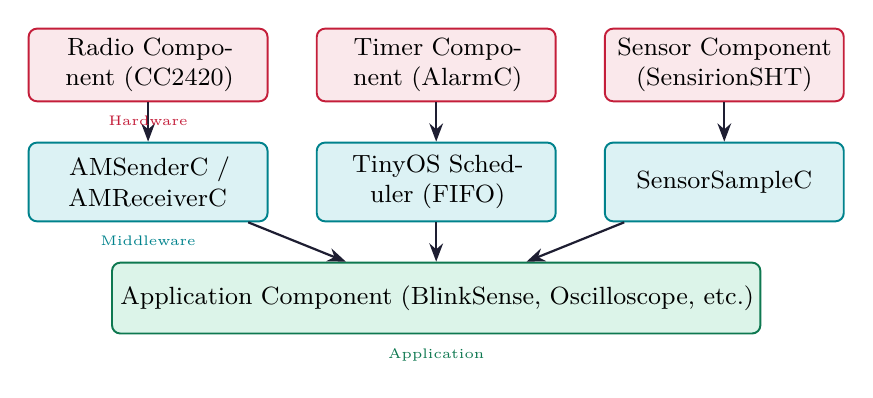
\begin{tikzpicture}[node distance=0.5cm and 0.9cm,
  comp/.style={rectangle, draw=myteal, fill=hdrteal, text width=2.8cm,
    align=center, minimum height=1.0cm, font=\small, rounded corners=3pt, line width=0.7pt},
  hwcomp/.style={rectangle, draw=myred, fill=hdrred, text width=2.8cm,
    align=center, minimum height=0.9cm, font=\small, rounded corners=3pt, line width=0.7pt},
  appcomp/.style={rectangle, draw=mygreen, fill=hdrgreen, text width=2.8cm,
    align=center, minimum height=0.9cm, font=\small, rounded corners=3pt, line width=0.7pt}]

  % Hardware components
  \node[hwcomp] (radio) {Radio Component (CC2420)};
  \node[hwcomp, right=0.6cm of radio] (timer) {Timer Component (AlarmC)};
  \node[hwcomp, right=0.6cm of timer] (sens) {Sensor Component (SensirionSHT)};

  % Middleware / OS
  \node[comp, below=0.5cm of radio] (mac) {AMSenderC / AMReceiverC};
  \node[comp, below=0.5cm of timer] (sched) {TinyOS Scheduler (FIFO)};
  \node[comp, below=0.5cm of sens] (sample) {SensorSampleC};

  % Application
  \node[appcomp, below=0.5cm of sched, text width=8cm] (app) {Application Component (BlinkSense, Oscilloscope, etc.)};

  % Connections
  \draw[arrow] (radio) -- (mac);
  \draw[arrow] (timer) -- (sched);
  \draw[arrow] (sens) -- (sample);
  \draw[arrow] (mac) -- (app);
  \draw[arrow] (sched) -- (app);
  \draw[arrow] (sample) -- (app);

  \node[font=\tiny, color=myred, below=0.05cm of radio] {Hardware};
  \node[font=\tiny, color=myteal, below=0.05cm of mac] {Middleware};
  \node[font=\tiny, color=mygreen, below=0.05cm of app] {Application};
\end{tikzpicture}
\end{tcolorbox}

% ===============================================================================
\section{nesC Programming Language}
% ===============================================================================

\begin{tcolorbox}[defbox, title={\textbf{nesC --- Definition}}]
\textbf{nesC} (network embedded systems C) is a component-based, event-driven extension of the C programming language designed specifically for TinyOS and sensor network applications. It provides the \textbf{component model}, \textbf{interface} declarations, and \textbf{wiring} syntax to compose TinyOS applications from reusable modules.
\end{tcolorbox}

\subsection{Key nesC Concepts}

\subsubsection*{1. Interfaces}
An \textbf{interface} defines a set of bidirectional operations:
\begin{itemize}[leftmargin=*, itemsep=2pt]
  \item \textbf{Commands:} Called by the user of the interface (top-down call). E.g., \texttt{AMSend.send()}.
  \item \textbf{Events:} Signaled by the provider of the interface (bottom-up notification). E.g., \texttt{AMSend.sendDone()}.
\end{itemize}

\subsubsection*{2. Components}
Two types of components:
\begin{itemize}[leftmargin=*, itemsep=2pt]
  \item \textbf{Module:} Implements an interface; contains C-like code for commands and event handlers.
  \item \textbf{Configuration:} Wires components together (no code, only connections).
\end{itemize}

\subsubsection*{3. Split-Phase Operations}
Long-running operations (radio TX, ADC conversion) are split into:
\begin{itemize}[itemsep=2pt]
  \item \textbf{Initiation:} Call a command (e.g., \texttt{call AMSend.send(...)}) --- returns immediately.
  \item \textbf{Completion:} An event is signaled when done (e.g., \texttt{event AMSend.sendDone(...)}). No blocking.
\end{itemize}

\subsubsection*{4. Tasks}
\begin{itemize}[itemsep=2pt]
  \item Deferred computation: \texttt{post myTask();} schedules a task in the FIFO queue.
  \item Tasks run to completion; they cannot be preempted by other tasks (only by events/interrupts).
\end{itemize}

\subsubsection*{5. Atomicity and Race Conditions}
\begin{itemize}[itemsep=2pt]
  \item \texttt{atomic \{ ... \}} block: disables interrupts for short, critical sections.
  \item nesC compiler performs a \textbf{race condition analysis} at compile time to flag potential data races between tasks and events.
\end{itemize}

\subsection{TinyOS vs Linux vs RTOS}

\par\noindent
{\renewcommand{\arraystretch}{1.5}%
\begin{tabularx}{\linewidth}{|B{2.8cm}|Y|Y|Y|}
\hline
\textbf{Feature} & \textbf{TinyOS} & \textbf{Linux} & \textbf{RTOS (FreeRTOS)} \\
\hline
\textbf{RAM} & 2--10 KB & 10s MB & 5--50 KB \\
\hline
\textbf{Scheduling} & Event-driven & Preemptive & Preemptive \\
\hline
\textbf{Tasks} & FIFO, non-preemptive & Preemptable threads & Priority-based tasks \\
\hline
\textbf{Language} & nesC (C extension) & C & C \\
\hline
\textbf{Energy mgmt} & First-class & Limited & Good \\
\hline
\textbf{Blocking calls} & Not allowed & Allowed & Allowed \\
\hline
\textbf{Use case} & WSN motes (8/16-bit MCU) & General-purpose (Raspberry Pi) & IoT/embedded (ARM Cortex-M) \\
\hline
\end{tabularx}}

% ===============================================================================
\newpage
\begin{center}
  {\large\bfseries\color{myred} Quick Revision --- Module 5}\\[3pt]
  {\small\color{mydark} Design Principles, Gateway Concepts \& TinyOS/nesC $|$ PE-EC703B}
\end{center}
\noindent{\color{myred}\rule{\linewidth}{1.2pt}}
\vspace{4pt}
% ===============================================================================

\begin{tcolorbox}[formulabox, title={\textbf{Key Concepts at a Glance}}]
\renewcommand{\arraystretch}{1.35}
\begin{tabularx}{\linewidth}{B{5.0cm} X}
6LoWPAN Compression & IPv6 (40 B) + UDP (8 B) $\rightarrow$ IPHC compressed header ($\leq$ 6 B) \\[4pt]
IEEE 802.15.4 Payload & Max payload: 127 B (PHY layer), 102 B (MAC layer after headers) \\[4pt]
IPv6 MTU size & 1280 B \quad ($\Rightarrow$ 6LoWPAN fragmentation required for WPAN link) \\[4pt]
CoAP Fixed Header & Only 4 bytes \quad (vs HTTP which requires $>100$ bytes header) \\[4pt]
TinyOS Scheduler & FIFO task queue; non-preemptive tasks; events interrupt tasks \\[4pt]
nesC Split-Phase & \texttt{call Iface.start()} initiates; \texttt{event Iface.startDone()} signals completion \\[4pt]
Gateway Function & Protocol translation (ZigBee $\leftrightarrow$ TCP/IP), buffering, security bridging
\end{tabularx}
\end{tcolorbox}

\begin{tcolorbox}[defbox, title={\textbf{One-Line Definitions}}]
\begin{itemize}[leftmargin=*, itemsep=3pt]
  \item \textbf{WSN Gateway:} Bridges IEEE 802.15.4/ZigBee WSN to Internet via protocol translation and data formatting.
  \item \textbf{6LoWPAN:} IETF adaptation layer running IPv6 over IEEE 802.15.4 via header compression and fragmentation.
  \item \textbf{CoAP:} Lightweight REST protocol over UDP for constrained IoT devices; the ``HTTP of IoT.''
  \item \textbf{RPL:} IETF routing protocol for 6LoWPAN; builds a DODAG (Destination-Oriented DAG) for uplink and downlink routing.
  \item \textbf{MQTT:} Publish-subscribe message protocol over TCP; broker buffers messages for offline sensor nodes.
  \item \textbf{TinyOS:} Event-driven, component-based OS for sensor motes; $<$15 KB footprint; non-preemptive.
  \item \textbf{nesC:} System programming language for TinyOS; extends C with components, interfaces, and wiring.
  \item \textbf{Split-phase:} Operation model where a command initiates and an event signals completion; no blocking.
\end{itemize}
\end{tcolorbox}

\begin{tcolorbox}[exambox, title={\textbf{Frequently Asked / Viva Questions}}]
\begin{enumerate}[topsep=0pt, label=\textbf{Q\arabic*.}, itemsep=5pt]
  \item \Q{What are the key design principles for WSN?}
  Eight principles: (1) Energy efficiency first; (2) In-network processing/aggregation; (3) Cross-layer design; (4) Self-organization and adaptivity; (5) Collaboration and redundancy; (6) Data-centric communication; (7) Quality/fidelity trade-off; (8) Security by design. Energy is always the primary constraint driving all design decisions.

  \item \Q{What is a WSN gateway? What are its functions?}
  A WSN gateway bridges the sensor network (IEEE 802.15.4/ZigBee) to the Internet. Functions: (1) Protocol translation (ZigBee $\leftrightarrow$ TCP/IP); (2) Data buffering; (3) Data formatting (JSON/MQTT); (4) Security bridging (WSN AES $\leftrightarrow$ internet TLS); (5) Task/query injection into WSN; (6) Network management and monitoring.

  \item \Q{What is 6LoWPAN? Why is it needed?}
  6LoWPAN (IPv6 over Low-Power WPANs) is an adaptation layer (RFC 4944) enabling IPv6 packets to run over IEEE 802.15.4. It is needed because: IPv6 header = 40 B but 802.15.4 payload = 102 B (only 62 B left for UDP+data after raw IPv6). 6LoWPAN compresses IPv6+UDP to $\leq$ 6 B using IPHC and fragments large packets, enabling IP-native WSN nodes.

  \item \Q{What is CoAP? How does it differ from HTTP?}
  CoAP (Constrained Application Protocol) is a lightweight REST protocol for IoT running over UDP. Differences from HTTP: runs over UDP (not TCP), has only 4-byte fixed header (vs 100+ bytes in HTTP), uses binary encoding (not text), includes built-in reliability (CON/ACK), supports observe mode (server push). Designed for $< 10$ KB RAM devices.

  \item \Q{Explain TinyOS architecture.}
  TinyOS is an event-driven, component-based OS. Architecture: (1) \textbf{Components} --- modules (implement code) and configurations (wire components); (2) \textbf{Interfaces} --- define commands (calls) and events (callbacks); (3) \textbf{Scheduler} --- FIFO task queue; tasks run to completion; events can interrupt tasks; (4) \textbf{Split-phase} --- no blocking calls; operations initiated by commands, completed by events. Footprint: $<$15 KB Flash, $<$4 KB RAM.

  \item \Q{What is nesC? Explain its key concepts.}
  nesC (network embedded systems C) is a component-based C extension for TinyOS. Key concepts: (1) \textbf{Interface} --- defines commands (top-down) and events (bottom-up); (2) \textbf{Module} --- implements an interface; (3) \textbf{Configuration} --- wires components at compile time; (4) \textbf{Split-phase} --- non-blocking; (5) \textbf{Tasks} --- deferred computation posted to FIFO queue; (6) \textbf{Atomic} --- interrupt-disable for race-condition-free critical sections.

  \item \Q{What is a split-phase operation in TinyOS? Give an example.}
  A split-phase operation separates initiation from completion: the call initiates an operation and returns immediately (no blocking); an event fires when the operation is done. Example: \texttt{call AMSend.send(msg)} starts radio transmission and returns immediately. When TX is done, \texttt{event AMSend.sendDone(msg, error)} is triggered for the application to handle success/failure.

  \item \Q{Compare TinyOS, Linux, and FreeRTOS for WSN use.}
  TinyOS: 2--10 KB RAM, event-driven, FIFO non-preemptive tasks, designed for 8/16-bit WSN motes. Linux: 10s MB RAM, preemptive threads, general-purpose, too heavy for motes. FreeRTOS: 5--50 KB RAM, preemptive priority tasks, good energy management, targets ARM Cortex-M IoT --- middle ground. TinyOS is best for truly constrained WSN nodes; FreeRTOS for richer IoT devices.

  \item \Q{What is RPL routing protocol?}
  RPL (Routing Protocol for Low-Power and Lossy Networks, RFC 6550) is the IETF standard routing protocol for 6LoWPAN. It builds a \textbf{DODAG} (Destination-Oriented Directed Acyclic Graph) rooted at the sink. Uplink (sensor to sink) follows parent links up the DAG. Downlink (Internet to sensor) uses source routing. Nodes use an \textbf{Objective Function} (e.g., ETX = Expected Transmissions, minimize energy) to select parents.

  \item \Q{What is the need for Internet-to-WSN downlink communication?}
  Internet-to-WSN downlink enables: (1) \textbf{Task injection} --- issuing queries like ``measure temperature every 5 s for 1 hour''; (2) \textbf{Actuator control} --- turning on/off actuators (valves, lights) from remote; (3) \textbf{Configuration updates} --- changing sampling rate, thresholds; (4) \textbf{Firmware over-the-air (FOTA)} --- updating node software remotely. Challenges: sleeping nodes, addressing, reliability over lossy links.

  \item \Q{What is MQTT and how is it used in WSN integration?}
  MQTT (Message Queuing Telemetry Transport) is a lightweight publish-subscribe protocol over TCP. A \textbf{broker} manages topics. Sensor nodes (via gateway) publish to topics (e.g., \texttt{sensor/room1/temp}); Internet applications subscribe. The broker buffers messages for offline subscribers. Advantages: very small packet overhead (2-byte header), store-and-forward for intermittent connectivity.

  \item \Q{What is cross-layer design in WSN?}
  Cross-layer design violates the traditional layered (OSI) model by allowing information to be shared between non-adjacent layers (e.g., MAC, routing, application) for joint optimization. Example: LEACH combines MAC (TDMA scheduling), network layer (clustering), and application (data rate adaptation) into one cross-layer protocol. Benefit: significant energy savings over pure layered design. Drawback: reduces modularity and reusability.
\end{enumerate}
\end{tcolorbox}

\begin{tcolorbox}[tikzbox, title={\textbf{Summary: WSN OS and Internet Integration}}]
\par\noindent
{\renewcommand{\arraystretch}{1.4}%
\begin{tabularx}{\linewidth}{|B{2.6cm}|Y|Y|}
\hline
\textbf{Component} & \textbf{Role} & \textbf{Key Feature} \\
\hline
TinyOS & WSN embedded OS & Event-driven, $<$15 KB, non-preemptive \\
\hline
nesC & Programming language & Components, interfaces, split-phase \\
\hline
Gateway & WSN-Internet bridge & Protocol translation, buffering \\
\hline
6LoWPAN & Adaptation layer & IPv6 over 802.15.4, header compression \\
\hline
CoAP & Application protocol & REST over UDP, 4B header \\
\hline
RPL & Routing protocol & DODAG for 6LoWPAN mesh \\
\hline
MQTT & Message protocol & Pub-sub, broker, store-and-forward \\
\hline
\end{tabularx}}
\end{tcolorbox}

\end{document}
